\chapter{人体行为识别系统设计介绍}
\par 针对基于智能手机的行为识别的研究,本文所提出了的两层多策略的行为识别方案框架以及降低识别能耗的最佳策略动态调整方法,为验证它们的有效性和实用性,本文实现了一款可以运行于Android手机操作系统上的行为识别应用。之所以选择Android手机操作系统,一方面是因为它是开源且成熟的智能手机操作系统,提供了丰富的应用编程接口,基于该操作系统的应用较多,基于Android系统开发行为识别应用容易开发实现。另一方面是因为Android操作系统的市场占有量最高,是目前应用最为广泛的手机操作系统,因此基于Android系统开发行为识别应用,也更具有代表性。
\par 本文所实现的行为识别应用可以使用智能手机内置传感器获取关于人体行为的相关传感器数据,并通过已经实现的分类算法对用户当前行为作出识别判断。与此同时,该应用还具有与远端服务器通信的功能,可以保存用户运动数据以及查询用户的历史运动数据等,从而构成一套较为完整的人体行为识别系统。行为识别应用的框架结构如图所示。
%应用框架结构
\begin{figure}[ht]
\centering
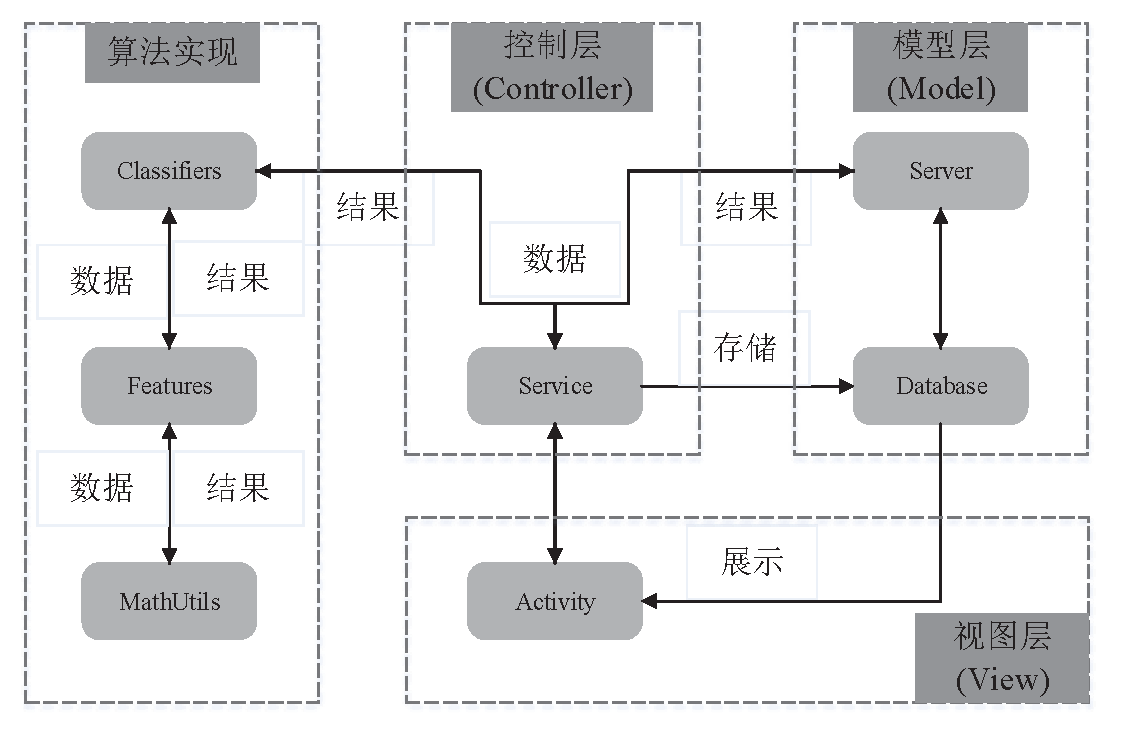
\includegraphics[width = 0.8\textwidth]{app_framework.eps}
\caption{最佳策略的动态调整方案框图}
\end{figure}
\par 行为识别应用共分为控制层,分类算法,模型层和视图层四部分。其中,由于本文的研究重点是基于智能手机的行为识别算法以及降低能耗的最佳策略调整方法,因此本文将应用框架的分类算法实现部分从模型层中分离出来单独介绍。控制层主要负责传感器的数据获取以及协调其他各部分的功能并与之通信,模型层主要负责数据的加载与保存,以及本地数据与远端服务器数据的同步等,视图层则只负责与用户的交互以及识别结果的展示。本章将从这四部分介绍人体行为识别系统的具体功能。
\section{控制层部分}
\par 行为识别应用的控制层主要由一个Android系统中的Service组成,主要负责数据获取以及统一协调其他功能模块两方面的功能。Service是Android操作系统中的重要组件之一,它没有可视化界面,是一种运行于后台的服务程序,主要负责不需要用户交互的长期运行任务。本文中的应用程序使用Service主要负责获取数据并协调控制其他功能模块。

\begin{enumerate}[(1)]
	\item 选择最佳策略
\end{enumerate}
\par 该部分实现本文提出的最佳策略动态调整方法,根据第四章中介绍的方法根据识别结果和行为转换矩阵计算下一窗口时间内最佳的识别策略,包括数据采样率,采样时间比例以及是否使用频域和自相关函数特征。策略的前两部分传递至数据获取功能模块,控制数据采集,后面两部分传递至算法实现部分,控制特征选择范围。
\begin{enumerate}[(2)]
	\item 获取传感器数据
\end{enumerate}
\par 数据获取功能模块主要负责采集以指定采样率和采样时间获取指定传感器的数据。一方面,在Service内部通过定义两个定时器控制采样时间,一个定时器负责控制数据窗口的大小也是行为识别判定一次的时间窗口大小,另一个定时器负责采样时间的比例,即控制传感器进入休眠状态,等待下一个窗口时间开始时唤醒。另一方面,在Service内部通过获取Android系统提供的SensorManager服务,统一管理传感器的操作,本文主要使用SensorManager获取指定传感器对象,同时根据两个定时器切换这些传感器工作和休眠的状态以及算法所设定的采样率。
\begin{enumerate}[(3)]
	\item 协调控制其他功能模块
\end{enumerate}
\par 除数据获取以外,控制层的Service的关键作用在于作为整个应用的枢纽,负责协调控制其他各个功能模块,包括将从传感器采集得到运动数据传递至算法实现部分对用户当前行为作出判断,并将识别结果送至视图层部分展示给用户,同时还负责将结果保存至本地数据库以及远端服务器等。其具体控制功能包括以下部分:
\begin{itemize}
	\item 控制算法实现部分:由定时器控制时间窗口大小,周期性地向算法实现部分传递传感器数据,并获取该窗口时间内的识别结果;
	\item 控制模型层部分:周期性地将识别结果保存至本地数据库,并在适当机会同步本地数据库与远端服务器的数据。
	\item 控制视图层部分:一方面负责接收视图层传递进来的用户交互事件命令,另一方面周期性地向视图层传递识别结果。
\end{itemize}
\section{分类算法实现部分}
\par 本部分主要实现第三章介绍的两层多策略的行为识别方案。该部分主要包括分类算法模块Classifier,特征提取与选择模块Features和数学工具模块MathUtils三部分,各部分的具体功能如下:
\begin{itemize}
	\item 分类算法模块:该部分负责接收Service传递进来的传感器数据并提供识别结果,内部包括实现的两层框架以及随机森林分类器,通过使用体征提取与选择模块提供的特征向量对当前时间窗口行为分类,计算最后识别结果;
	\item 特征提取与选择模块:该部分负责接收分类算法模块传递的传感器数据以及指定的特征序号计算指定特征,组成特征向量,返回至分类算法模块,用于行为分类;
	\item 数学工具:该部分负责提供各类数学计算工具,主要包括计算最值,均值,快速傅里叶变换,自相关函数等静态方法,为特征提取以及分类提供数学工具支持。
\end{itemize}
\section{模型层部分}
\par 由于本文将分类的业务逻辑已经单独提出在分类算法部分介绍,模型层部分则只需要负责对数据的存储和加载功能即可。对于数据的存储,本文使用Android系统内集成的SQLite数据库建立本地数据库存储行为数据。SQLite是一款轻型数据库,占用资源相对较少,常用于嵌入式设备。Android操作系统已经集成了SQLite数据库,使用该数据库可以方便地在手机端存储大量数据。Android操作系统提供有SQLiteOpenHelper工具类负责建立和更新数据库,同时也提供了一些编程接口,可以方便地使用SQL语句执行建表以及查询,插入,删除和更新数据等操作。
\par 本文所实现的应用需要存储的数据十分简单,只需要存储用户的行为信息即可。因此本应用所建立的数据库中包含用户表和行为表两个数据表。
\begin{itemize}
	\item 用户数据表$users$, 包括用户序号$user\_id$,用户名$user\_name$和密码$password$三个字段,用于记录用户信息以及登录过程的验证。
	\item 行为数据表$activities$,包括序号$\_id$, 用户序号$user\_id$,行为$activity$,时间$time$和是否已与服务器同步$is\_sync$五个字段,用于记录实时识别的行为信息。
\end{itemize}
\par 该应用的模型层部分对外提供操作数据库时的增删改查接口,便于其他部分对数据的操作。在识别过程中,由Service控制插入实时识别的行为数据,并且用户还可以通过视图层部分提供的用户界面操作控制数据的查询,删除和更新等。除此以外,Service还会在网络允许状态下负责本地数据库与远端服务器数据的同步。
\section{视图层部分}
\par 行为识别应用的界面层部分主要提供向用户展示识别结果以及为用户提供交互操作接口的功能。图\ref{screenshot1}(a)和(b)分别为手机应用的登录界面和初始化界面。用户登录以后进入初始化界面,此时应用会执行加载分类模型等一系列初始化操作,在初始化界面,开始按钮可以控制识别过程的开始与停止,查询按钮可以用于控制查询历史行为记录。
\begin{figure}[htb]
    \centering
    \subfigure[登录界面]{
    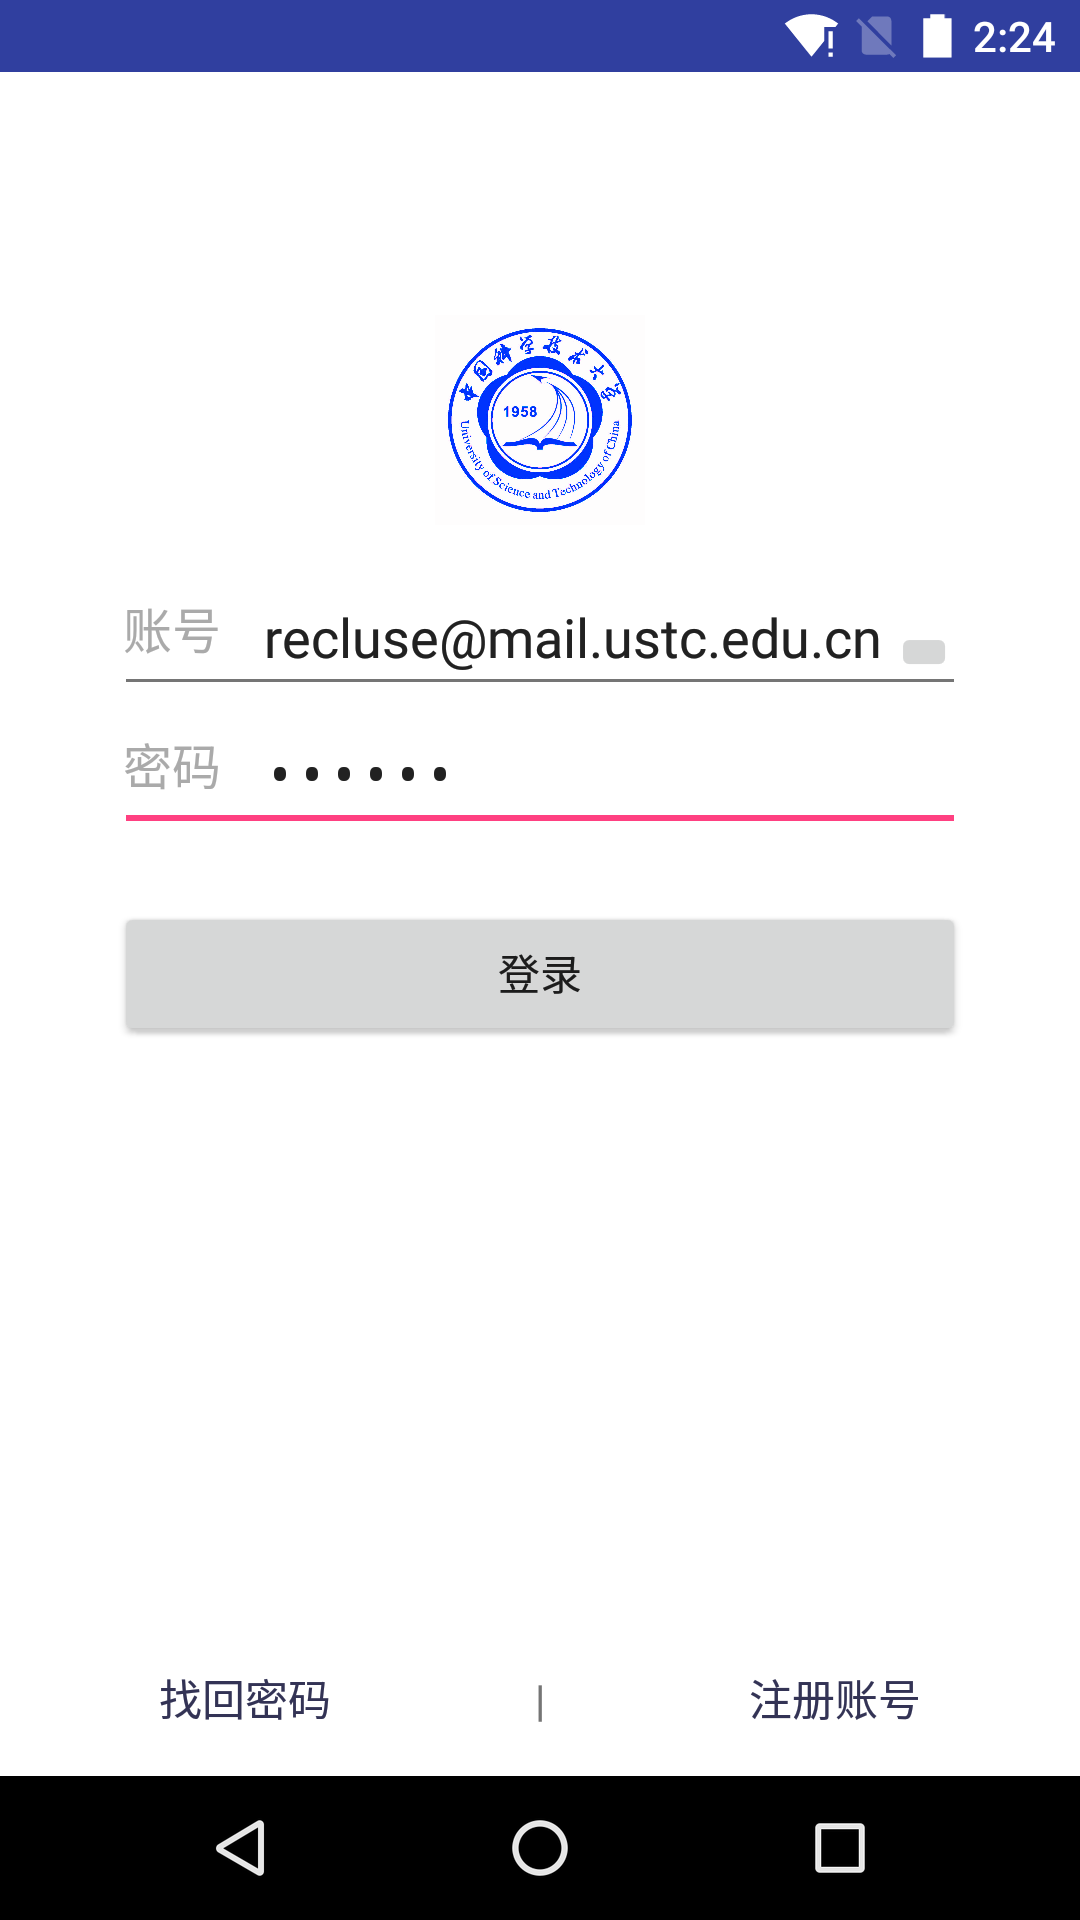
\includegraphics[width=0.3\textwidth]{login.png}}
    \subfigure[初始化界面]{
    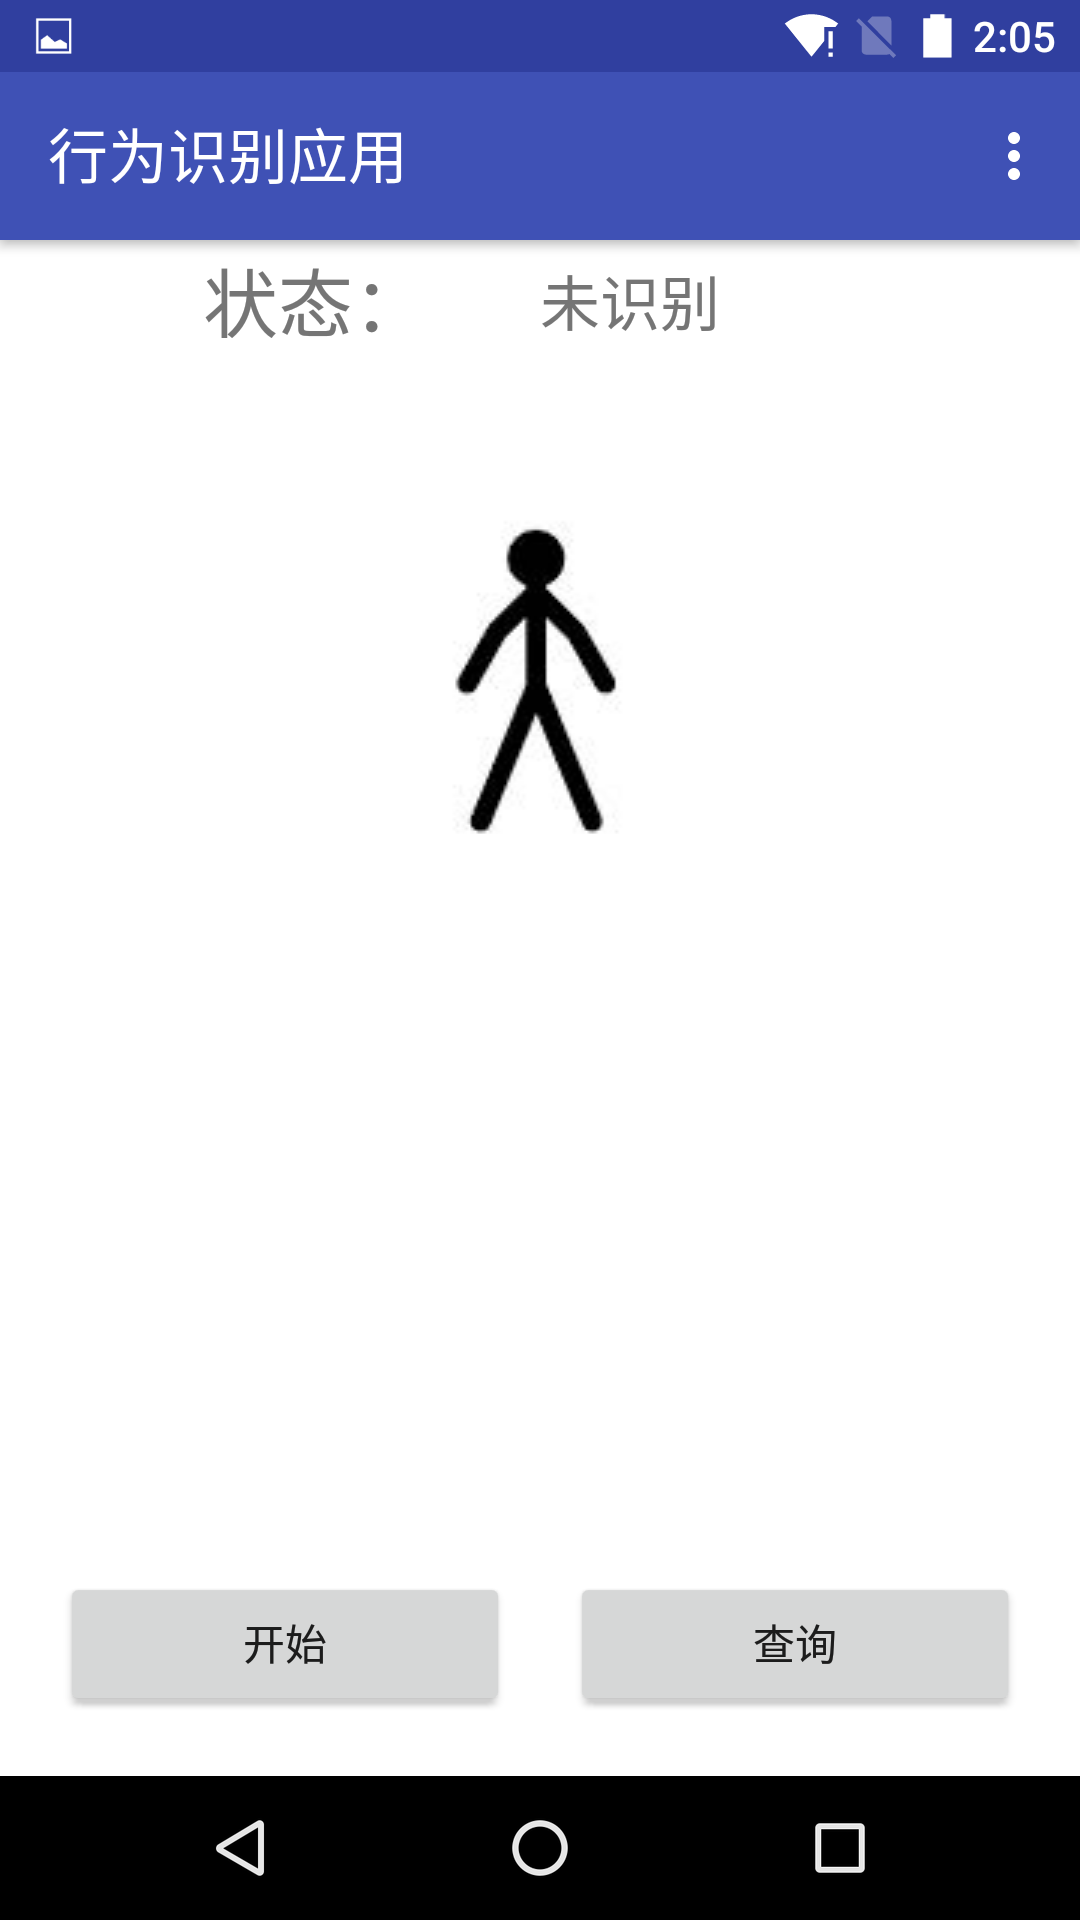
\includegraphics[width=0.3\textwidth]{init.png}}
    \caption{行为识别应用的部分界面}\label{screenshot1}
\end{figure}
\par 该行为识别应用提供两个展示识别结果的界面,一是如图\ref{screenshot2}(a)所示的行为GIF动画展示,二是如图\ref{screenshot2}(b)所示的以表格形式展示历史行为记录并随着识别过程实时更新曲线,通过查询/返回按钮可以控制两个界面的切换。同时该应用提供了历史记录的查询功能,通过菜单选项中提供的设置开始和结束时间,查询过去某一段时间的行为记录,记录以表格形式展示,在清除查询后表格恢复显示当前的实时行为记录。
\begin{figure}[htb]
    \centering
    \subfigure[行为GIF动画展示]{
    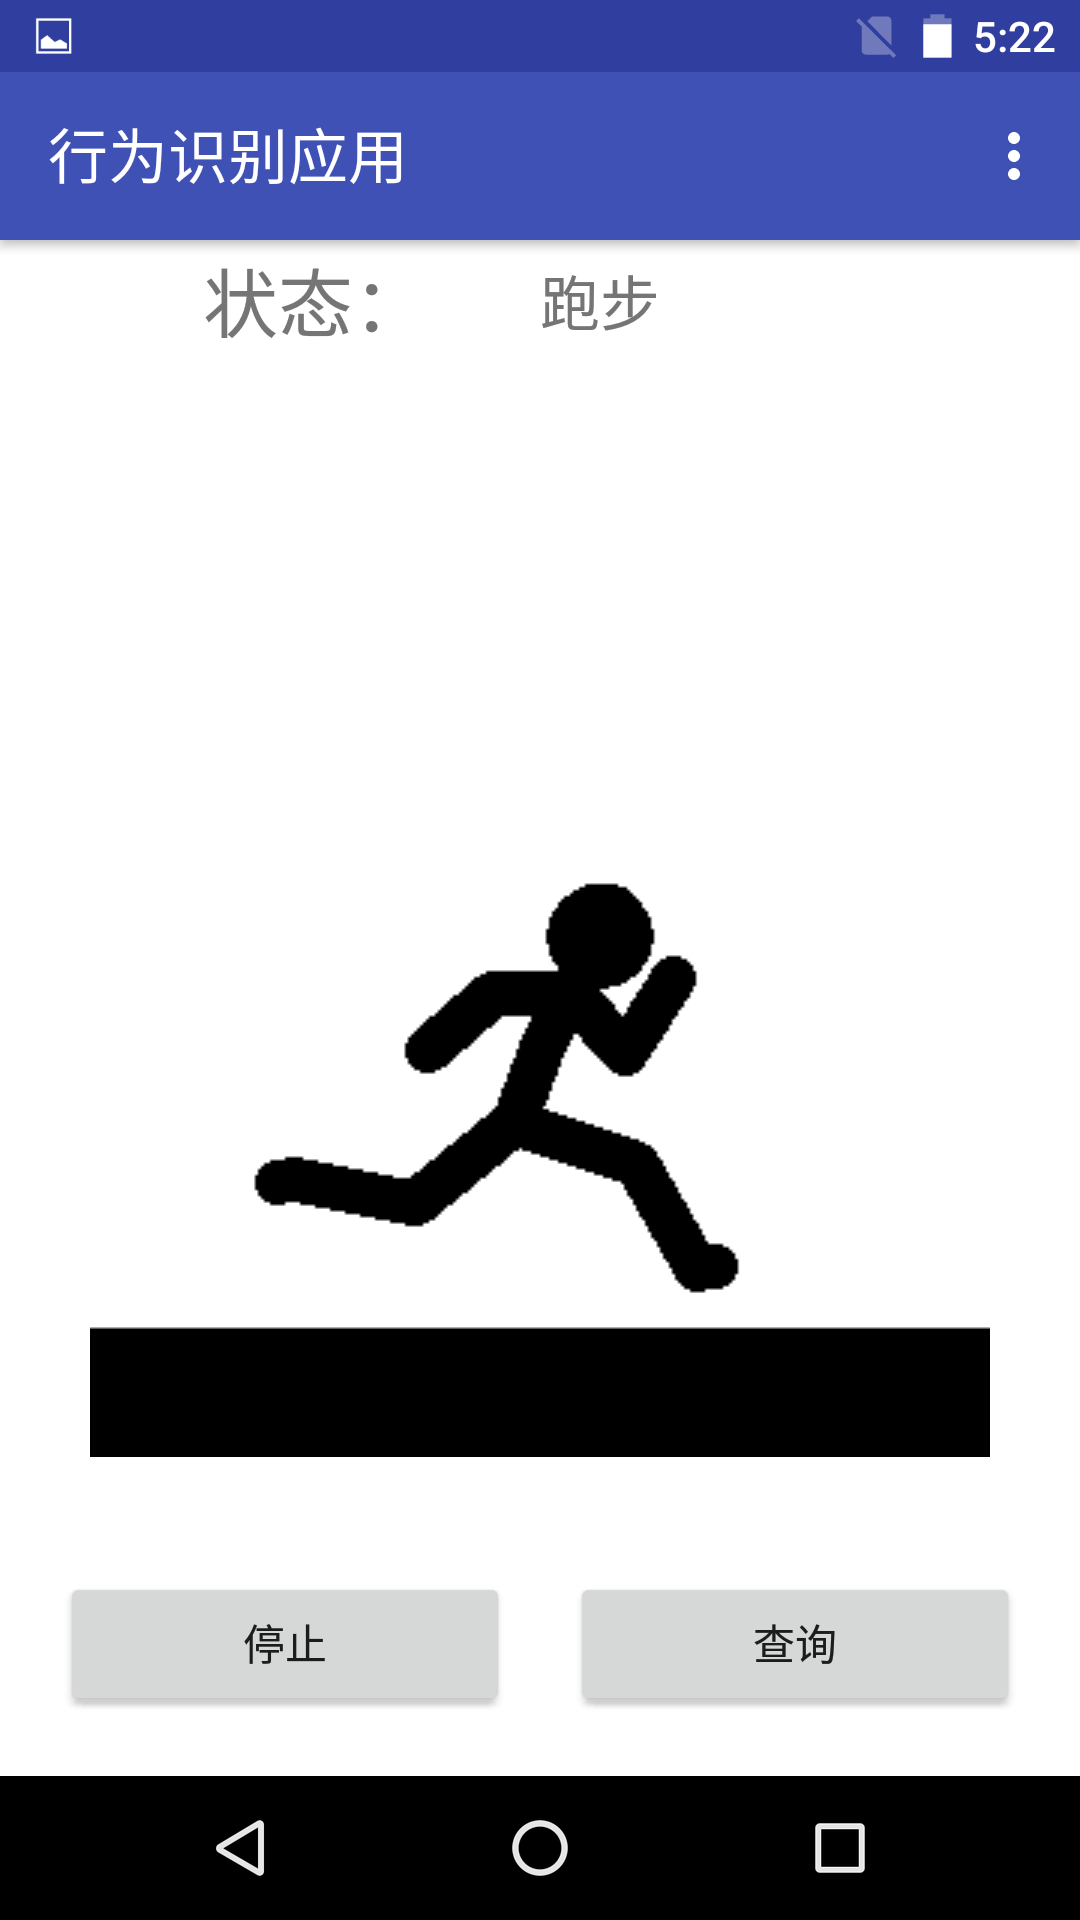
\includegraphics[width=0.23\textwidth]{run.png}}
    \subfigure[历史行为记录展示]{
    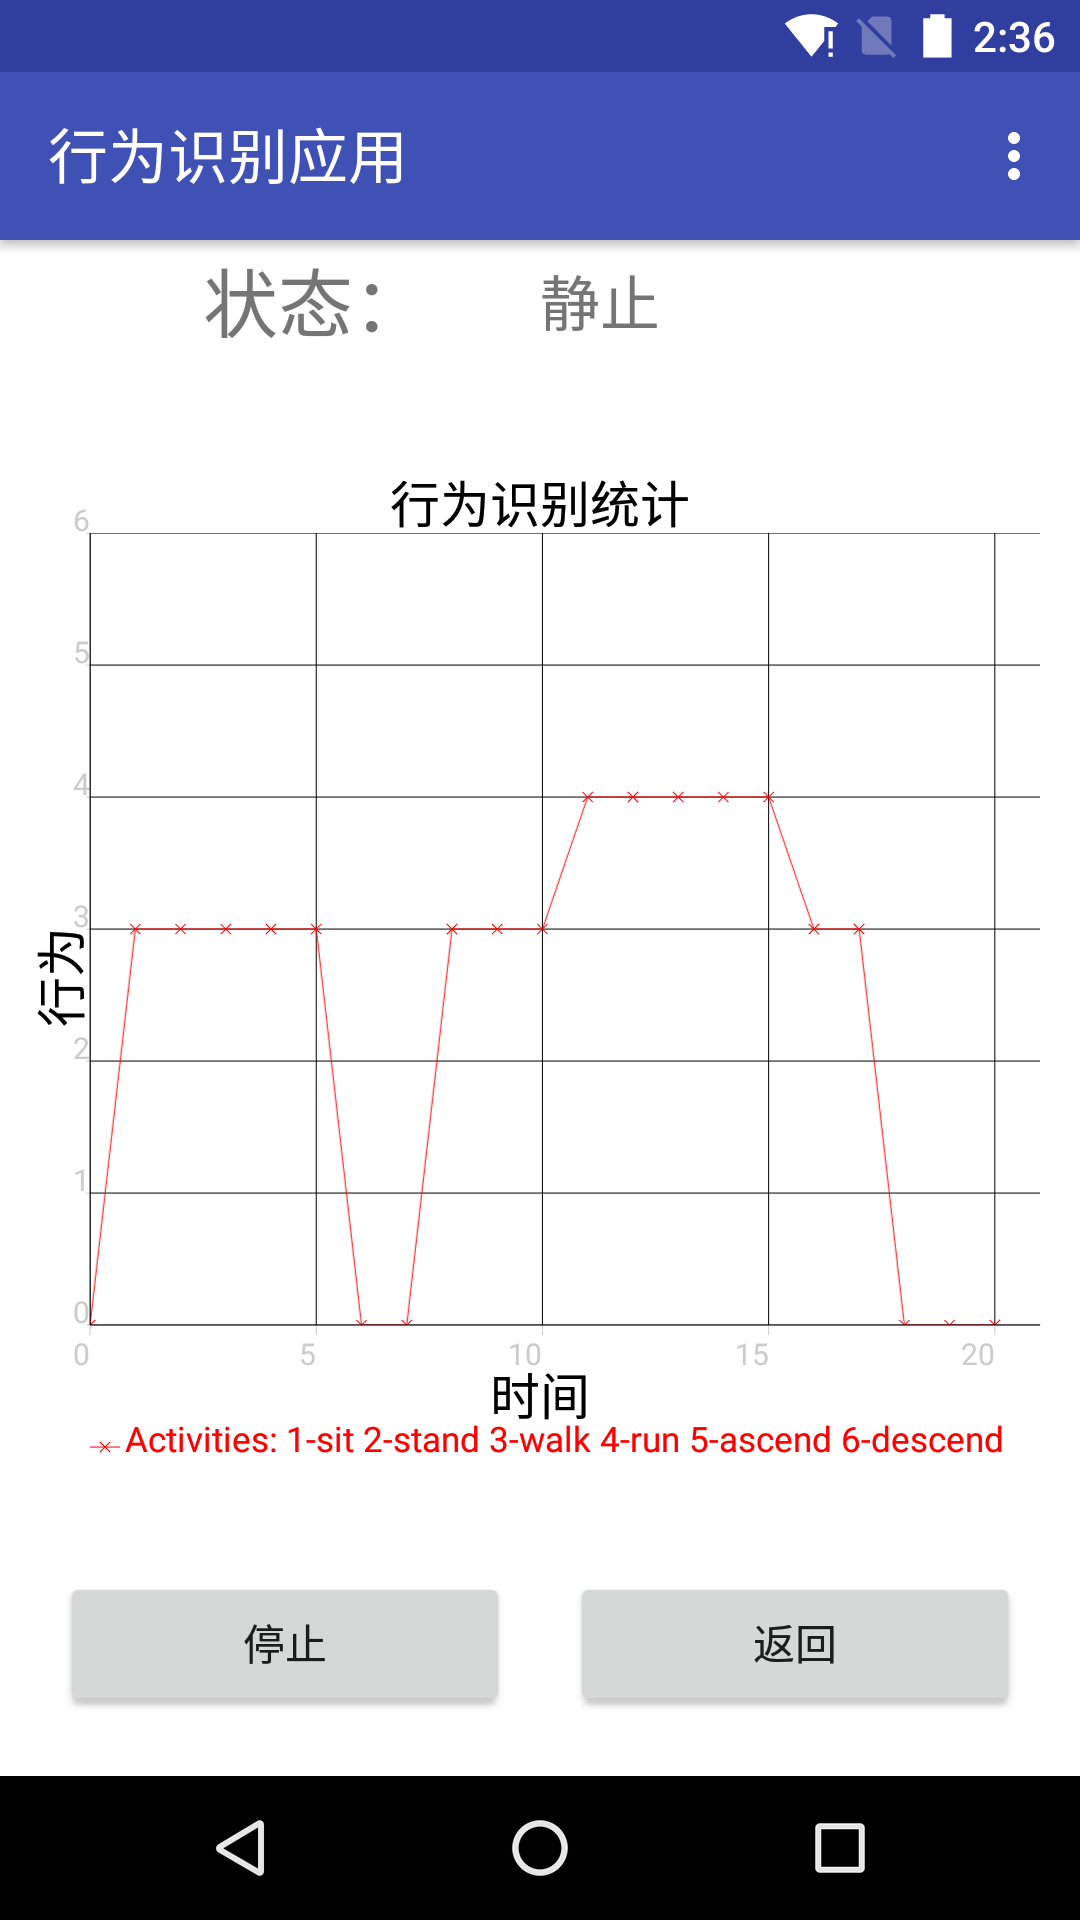
\includegraphics[width=0.23\textwidth]{query.png}}
    \subfigure[菜单选项]{
    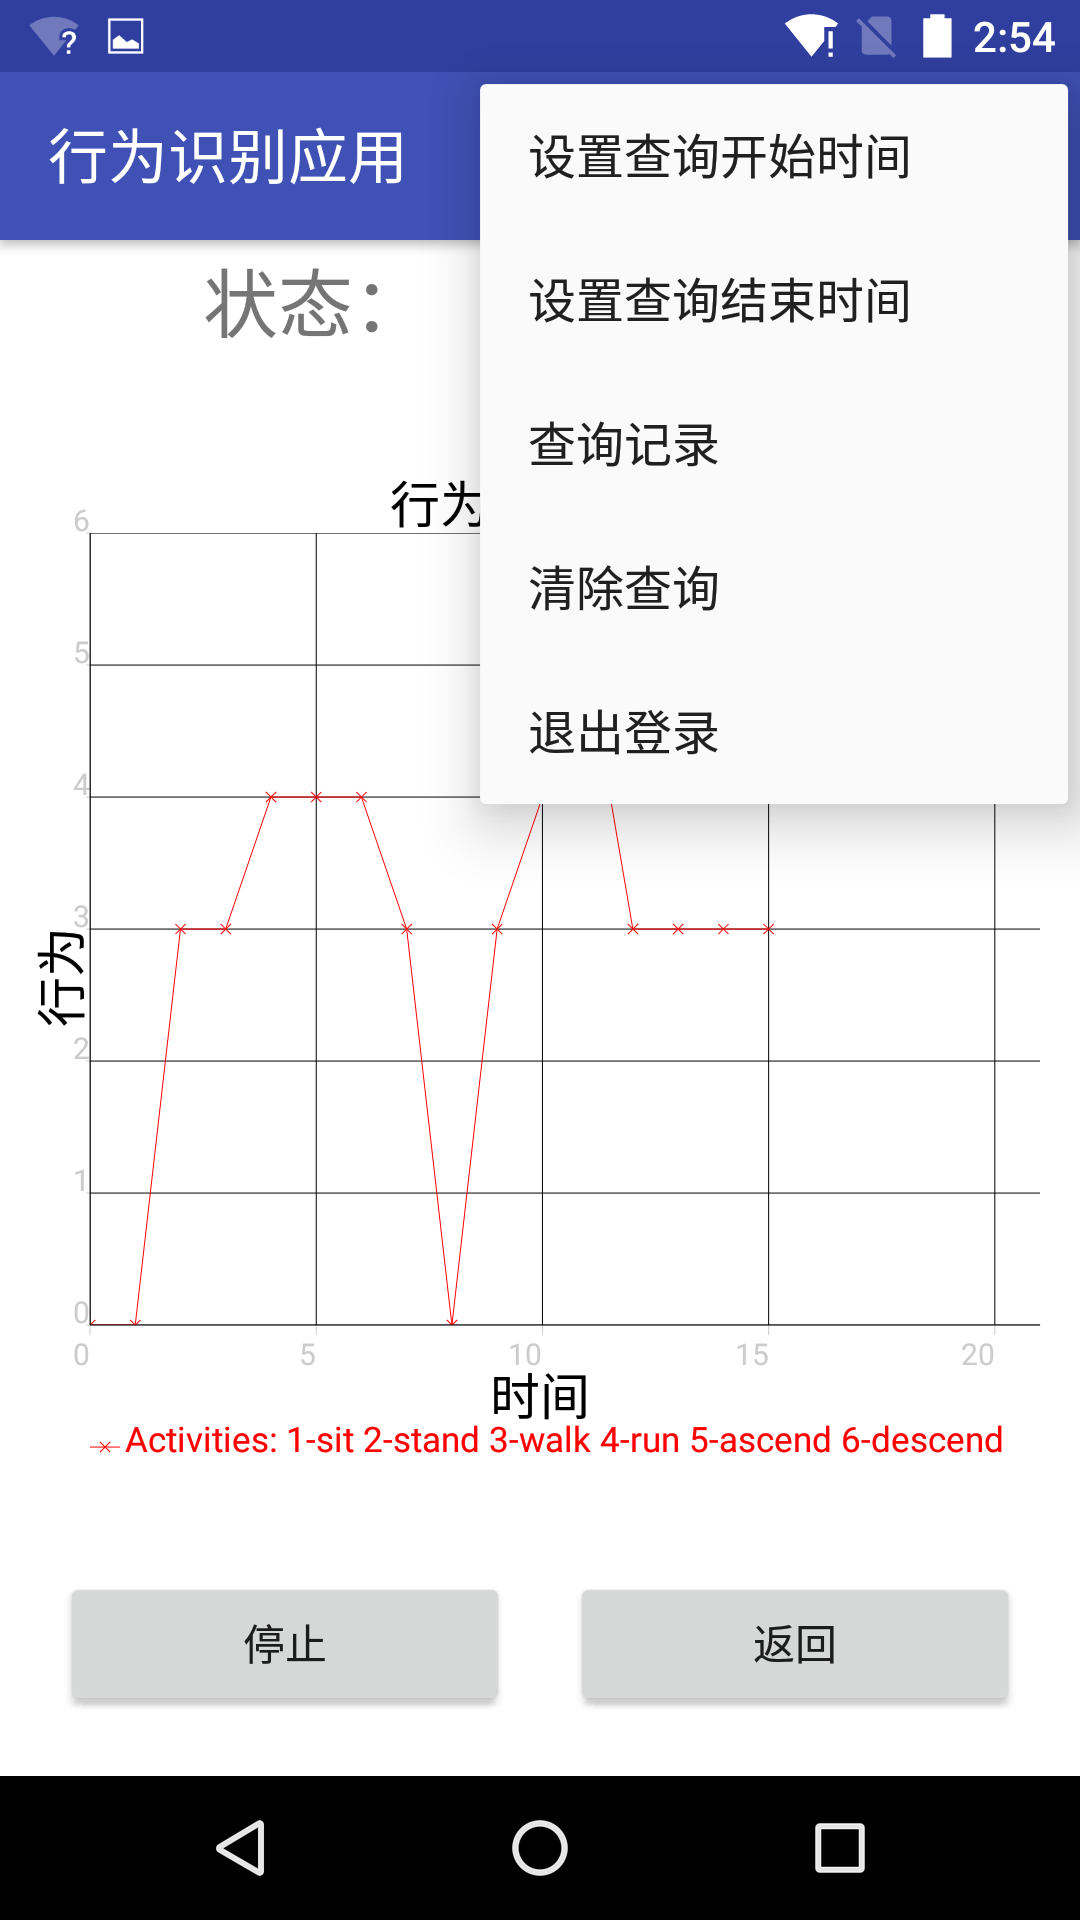
\includegraphics[width=0.23\textwidth]{menu.png}}
    \subfigure[时间设置对话框]{
    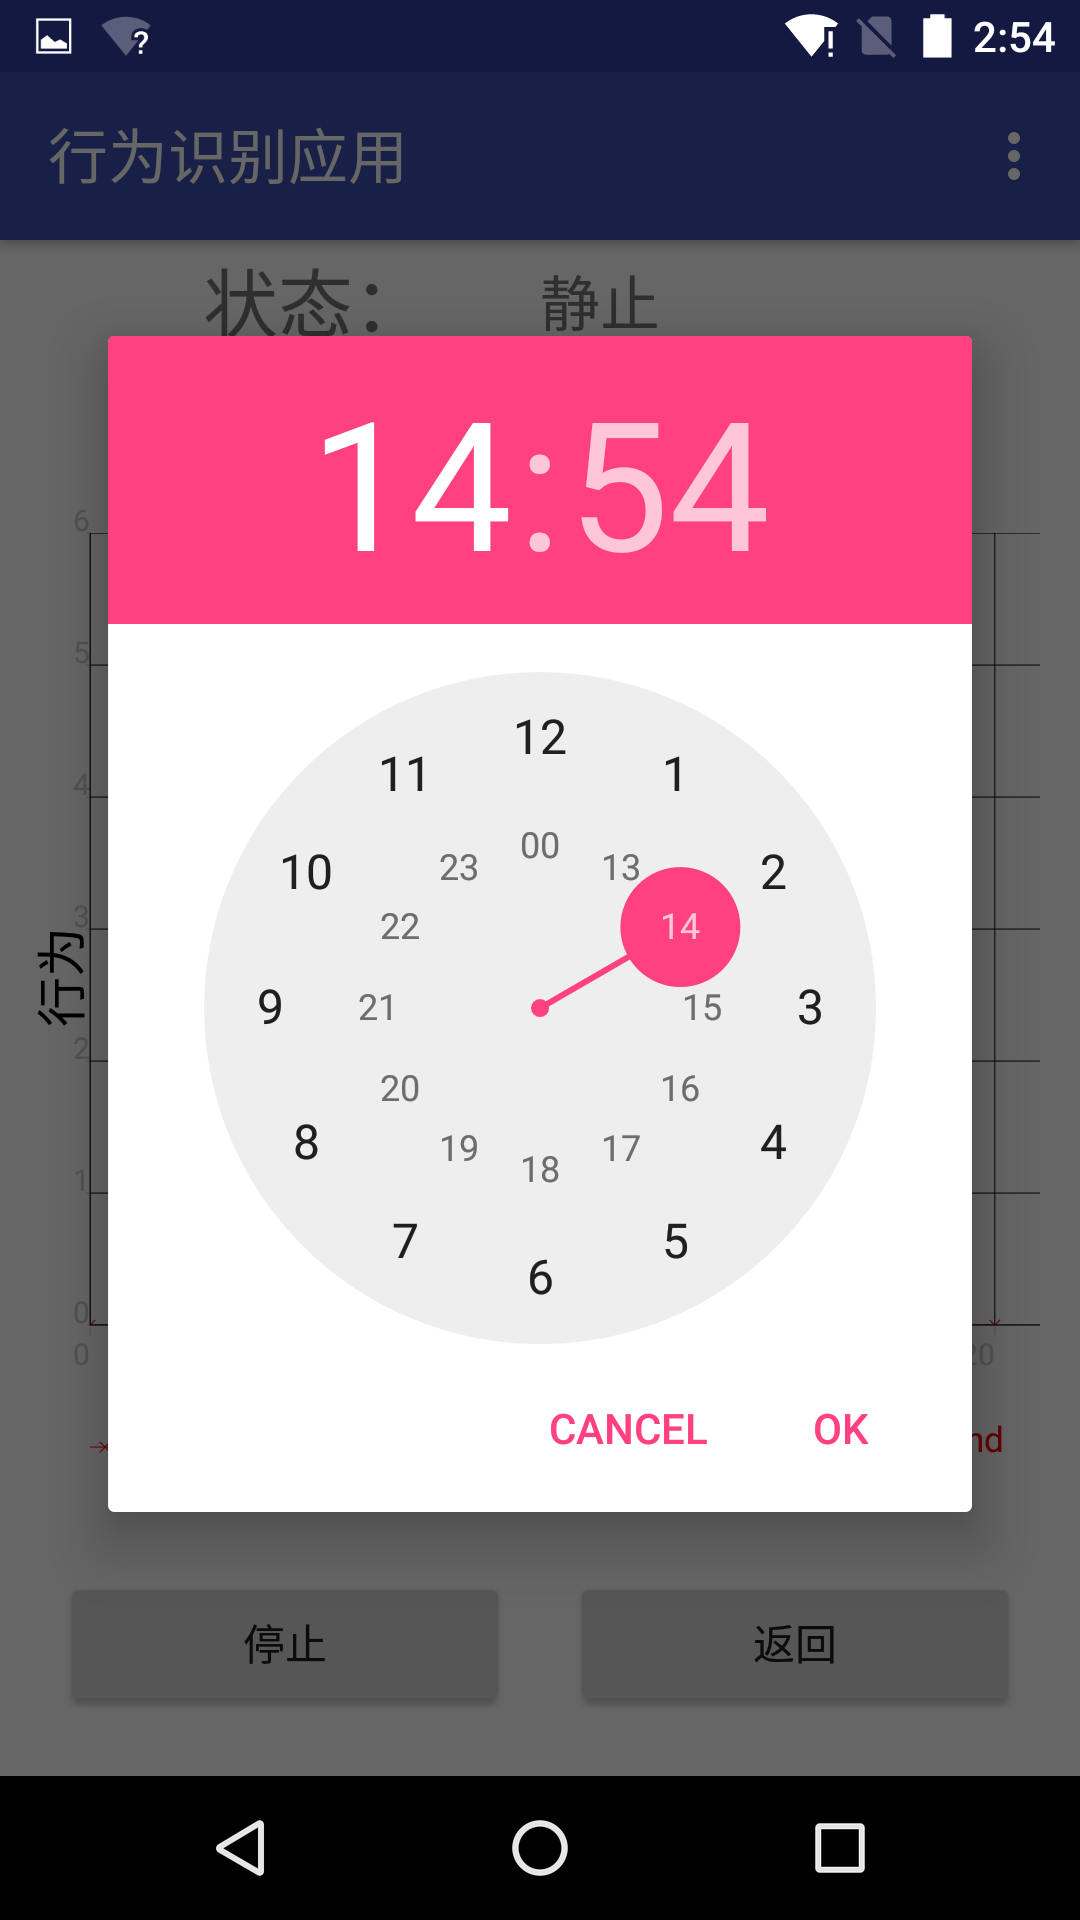
\includegraphics[width=0.23\textwidth]{dialog.png}}
    \caption{行为识别应用的部分界面}\label{screenshot2}
\end{figure}
\section{本章小结}
\par 本章首先介绍了本文所实现的人体行为识别系统的整体框架结构。然后从控制层部分,算法实现部分,模型层部分和视图层部分四个方面详细介绍了移动端行为识别应用的各部分组成和功能。
